\documentclass[notitlepage, a4paper, 11pt]{article}

\usepackage{geometry}
\geometry{
	a4paper,
	total={170mm,257mm},
	left=20mm,
	top=20mm,
}

\usepackage{gensymb}
\usepackage{wrapfig}
\usepackage{xcolor}
\usepackage{graphicx}
\usepackage{amsmath}
\usepackage{amssymb}
\usepackage{mathtools}
\usepackage{amsfonts}
\usepackage{listings}
\usepackage{xcolor}
\usepackage{minted}
\usepackage{tikz}
\usepackage[european resistors]{circuitikz}
\usepackage{caption}
\usepackage{subcaption}
\usepackage{hyperref}
\hypersetup{
	pdfborder = false,
	colorlinks=true,
	linkcolor=black,
	filecolor=black,      
	urlcolor=blue,
	pdftitle={Overleaf Example},
	pdfpagemode=FullScreen,
}
\title{Laplace Transform\\
	\large Laboratory III}
\author{Patrycja Nazim, Adrian Król, Gabriel Ćwiek, Kamil Chaj}
\date{}

\begin{document}
	\maketitle
	\section{Goal of the exercise}
	
	In this exercise, the primary goal is to validate the accuracy and effectiveness of the transient analysis approach using Laplace transformation. This method allows for the examination and understanding of the behavior of electrical circuits during the transient state. By measuring the voltages in both RC and RLC circuits that are subjected to a unit step input, we can observe and analyze the transient response of the circuits. This experimental verification provides valuable insights into the practical application and usefulness of the Laplace transformation technique in electrical circuit analysis.
	
	\section{Laplace Transform}
	Laplace transform is an integral transform that converts a function of a real variable(time domain) into a function of complex variable(frequency domain). It is powerful tool for solving differential equations, which turns ODEs into algebraic equations and convolution into multiplication. For function $x(t)$, the Laplace transform is the integral
	
	\begin{equation}
		\mathcal{L}[x(t)] = X(s) = \int_{0}^{\infty}x(t)e^{-st}dt
	\end{equation}
	
	Where $s = \sigma+j\omega$ $\quad \sigma,\omega\in \mathbb{R}$
	\\
	In order to get solution of differential equation solved in s-domain it is necessary to apply inverse Laplace transform which is given by following complex integral
	
	\begin{equation}
		f(t) = \mathcal{L}^{-1}[X(s)] = \dfrac{1}{2\pi j}\int_{c-j\infty}^{c+j\infty}F(s)e^{-st}ds
	\end{equation}
	
	Integrals like these can be quite difficult to solve, that is why lookup table of \href{https://en.wikipedia.org/wiki/Laplace_transform#Table_of_selected_Laplace_transforms}{Laplace transforms} and \href{https://en.wikipedia.org/wiki/Laplace_transform#Properties_and_theorems}{properties} can be very handy.
	\\ \\
	Moving to solving circuits using Laplace transform, there are two approaches, first is constructing differential equation in time domain describing circuit and then solve it using Laplace transform, or second option very similar to solving circuits in steady-state where all components are transformed to s-domain and at the end of calculation transform back to t-domain.
	
	\begin{equation}\label{eq:laplace-rules}
		R \xrightarrow{\mathcal{L}} R \quad C \xrightarrow{\mathcal{L}} \frac{1}{sC} \quad L \xrightarrow{\mathcal{L}} sL
	\end{equation}
	
	
	\section{Course of measurements}
		
		First we tested two circuits: low-pass and high-pass configuration of RC circuit and RLC circuts. After connecting osciloscope to the wave generator and prototype board, we generated square wave with $v_{pp}$ = 1V, $v_{offset}$ = .5V, frequency of 100Hz and duty cycle of 50\%. Then we read from the oscilloscope Voltage value at times 1$\tau$, 5$\tau$ and 10$\tau$ (where 10$\tau$ is just as fail-safe) and time when voltage reaches 10\% and 90\% of the highest value.
		
			\begin{figure}[H]
			\centering
			\begin{subfigure}{0.95\textwidth}
				\centering
				\begin{circuitikz}
					\ctikzset{bipoles/oscope/width=1.5}
					\ctikzset{bipoles/oscope/height=1}
					\draw [black, thick] (0, 0) rectangle (3, -2);
					\node [black, below] at (1.5, -2) {RC circuits};
					\draw [black, thick] (-3, 0) rectangle (-1, -1.5);
					\node [black, above] at (-2, 0) {\small Function Generator};
					\draw (1.5, 1.3) node[oscopeshape](O) {Oscilloscope};
					\node [bnc] at (-1.3, -0.75) (FG) {};
					\node [bnc, font=\tiny, xscale=-1, anchor=zero] at (1, -0.75) (CON1) {};
					\node [bnc, font=\tiny, rotate=90, anchor=zero, label position=45] at (2, -0.75) (CON2) {};
					\node [below, font=\tiny] at (1, -0.85) {CON2};
					\node [below, font=\tiny] at (2, -0.85) {CON1};
					\draw (O.in 1) node[bnc, anchor=zero, rotate=-90](IN1) {};
					\draw (O.in 2) node[bnc, anchor=zero, rotate=-90](IN2) {};
					\draw (FG.hot) to[short, -*] (-0.4, -0.75) -- (-0.4, 0.4) -- (1.08, 0.4) to (IN1.hot);
					\draw (CON1.hot) to[short] (-0.4, -0.75);
					\draw (CON2.hot) to[short] (2, 0.4) -- (1.92, 0.4) -- (IN2.hot);
				\end{circuitikz}
				\caption{Measurement setup}
			\end{subfigure}
			\begin{subfigure}{0.45\textwidth}
				\centering
				\begin{circuitikz}[scale = 0.7, transform shape]
					\draw (0,0) node[bnc](B1) {CON11}
					to[R, l=$R_{11}$, a=1.5k$\Omega$] (3,0)
					to[C, l2=$C_{11}$ and 47nF, l2 halign=c, l2 valign=c] (3,-2)
					node[ground] {}
					;
					\draw (3,0) 
					to[short] (4.5,0)
					node[bnc, xscale=-1](B2){\scalebox{-1}[1]{CON12}}
					;
					\draw node[ground] at (B1.shield) {};
					\draw node[ground] at (B2.shield) {};
				\end{circuitikz}
				\caption{Circuit A}
				\label{fig:Circuit A}
			\end{subfigure}
			\begin{subfigure}{0.45\textwidth}
				\centering
				\begin{circuitikz}[scale = 0.7, transform shape]
					\draw (0,0) node[bnc](B1) {CON21}
					to[C, l=$C_{21}$, a=10nF] (3,0)
					to[R, l2=$R_{21}$ and 1.5k$\Omega$, l2 halign=c, l2 valign=c] (3,-2)
					node[ground] {}
					;
					\draw (3,0) 
					to[short] (4.5,0)
					node[bnc, xscale=-1](B2){\scalebox{-1}[1]{CON21}}
					;
					\draw node[ground] at (B1.shield) {};
					\draw node[ground] at (B2.shield) {};
				\end{circuitikz}
				\caption{Circuit B}
				\label{fig:Circuit B}
			\end{subfigure}
			\caption{RC Circuits}
			\label{fig: Circuit}
		\end{figure}		
		
		For RLC circuits we tested two different resistances before RC circuit influence output characteristic. We measured response for 2 cases: Generator out resistance (50 $\Omega$) + resistance selected by jumper wire. In our case we tested jumper on 1.1k$\Omega$ resistance path and 3.3k$\Omega$. After that we checked response of the circuit:
		\begin{itemize}
			\item if response was sinusoid with decreasing amplitude - resustance was smaller then RC
			\item if response was exp. decay if R was higher
			\item if response was aperiodic critical waveform if resistance was equal RC
		\end{itemize}
		
	
	\begin{figure}[H]
		\centering
		\begin{subfigure}{0.45\textwidth}
			\centering
			\begin{circuitikz}[scale = 0.7, transform shape]
				\node [bnc] at (0,0) (CON41) {};
				\draw (CON41.hot) to[short, -*]
				(1,0) -- (3,0) to[nopb, l_=JP43] (4,0);
				\draw (1,0) -- (1,-2) to[R, l2=$R_{42}$ and $1.1k\Omega$, l2 halign=c, l2 valign=b] (3,-2)
				to[nopb, l_=JP42] (4,-2) -- (4, 0);
				\draw (1,-2) -- (1,-4) to[R, l2=$R_{41}$ and $3.3k\Omega$, l2 halign=c, l2 valign=b] (3,-4)
				to[nopb, l_=JP41] (4,-4) -- (4, -2);
				\draw (4,0) to[short, -*] (5,0)
				to[C, l2=$C_{41}$ and 33nF, l2 halign=c, l2 valign=c] (5,-2) 
				to[L, l2=$L_{41}$ and 10mH, l2 halign=c, l2 valign=c] (5,-4) node[ground] {};
				\draw (5, 0) to (6, 0) node[bnc, xscale=-1, anchor=zero](CON42){};
			\end{circuitikz}
			\caption{Measured Circuit}
		\end{subfigure}
		\hfill
		\begin{subfigure}{0.45\textwidth}
			\centering
			\begin{circuitikz}[scale = 0.8, transform shape]
				\ctikzset{bipoles/oscope/width=1.5}
				\ctikzset{bipoles/oscope/height=1}
				\draw [black, thick] (0, 0) rectangle (3, -3);
				\node [black, below] at (1.5, -3) {RC circuits};
				\draw [black, thick] (-3, 0) rectangle (-1, -1.5);
				\node [black, above] at (-2, 0) {\small Function Generator};
				\draw (4.5, 0.6) node[oscopeshape](O) {Oscilloscope};
				\node [bnc] at (-1.3, -0.75) (FG) {};
				\node [bnc, font=\tiny, xscale=-1, anchor=zero] at (0.5, -0.5) (CON1) {\ctikzflipx{CON1}};
				\node [bnc, font=\tiny] at (2.65, -0.5) (CON2) {CON2};
				\draw (CON2.left) to[short, -*] (1.5, -0.5);
				\draw (CON1.left) to[short, -*] (1.5, -0.5)
				to[C, bipoles/length=7mm] (1.5, -1.25)
				to[L, bipoles/length=10mm] (1.5, -2.5) node[tlground, scale=0.8]{};
				\draw (O.in 1) node[bnc, anchor=zero, rotate=-90](IN1) {};
				\draw (O.in 2) node[bnc, anchor=zero, rotate=-90](IN2) {};
				\draw (FG.hot) -- (-0.5, -0.75) -- (-0.5, -0.5) -- (CON1.hot);
				\draw (CON2.hot) -- (4.08, -0.5) -- (IN1.hot);
				\draw [black, ->](IN2.hot) -- (4.92, -1.35) -- (1.5, -1.35);
				\node [below] at (4.52, -1.3){probe};
			\end{circuitikz}
			\caption{Measurements setup}
		\end{subfigure}
		\caption{RLC circuit}
	\end{figure}

	\section{Theoretical calculations}
	For all calculations we used Matlab with Symbolic Math Toolbox. Source code can be found in Appendix. \ref{sec:appendix}
	\\ \\
	In all three circuit input voltage was square wave with 50\% duty cycle which can be described in time domain by
	
	\begin{equation}
		v_{in}(t) = V_{offset} \mathbf{1}(t) + V_{pp} \mathbf{1}(t-\frac{T}{2}) - V_{pp} \mathbf{1}(t-T)
	\end{equation}
	
	and in frequency domain by
	
	\begin{equation}
		V_{in}(s) = \mathcal{L}[v_{in}(t)] = \frac{V_{offset}}{s} + \dfrac{e^{-\frac{T}{2}s}}{s} - \dfrac{e^{-Ts}}{s}
	\end{equation}

	\subsection{Circuit A}

	First we need to transform circuit to s-domain according to \eqref{eq:laplace-rules}

	\begin{figure}[H]
		\centering
		\begin{circuitikz}[scale = 0.7, transform shape]
			\draw (0,0)
			to[R, l=$R_{11}$, *-] (3,0)
			to[C, l=$\dfrac{1}{sC_{11}}$] (3,-2)
			to[short, -*] (0, -2)
			;
			\draw (0, 0) to[open, v_<=$v_{in}$] (0, -2);
			\draw (3, 0)
			to[short, -*] (5, 0)
			to[open, v^<=$v_{out}$] (5, -2)
			to[short, *-] (3, -2);
		\end{circuitikz}
		\caption{Circuit A schematics}
	\end{figure}
	
	output voltag of circuit A can be described using simple voltage divider
	
	\begin{equation}
		V_{out}(s) = V_{in}(s) \dfrac{\frac{1}{sC_{11}}}{R_{11} +\frac{1}{sC_{11}}}
	\end{equation}
	
	after applying inverse Laplace transform to $v_{out}(s)$ we obtain below plot with marked $\tau$, 5$\tau$, 10$\tau$, 10\% and 90\% of output voltage.
	
	\begin{figure}[H]
		\centering
	\begin{subfigure}{0.6\textwidth}
	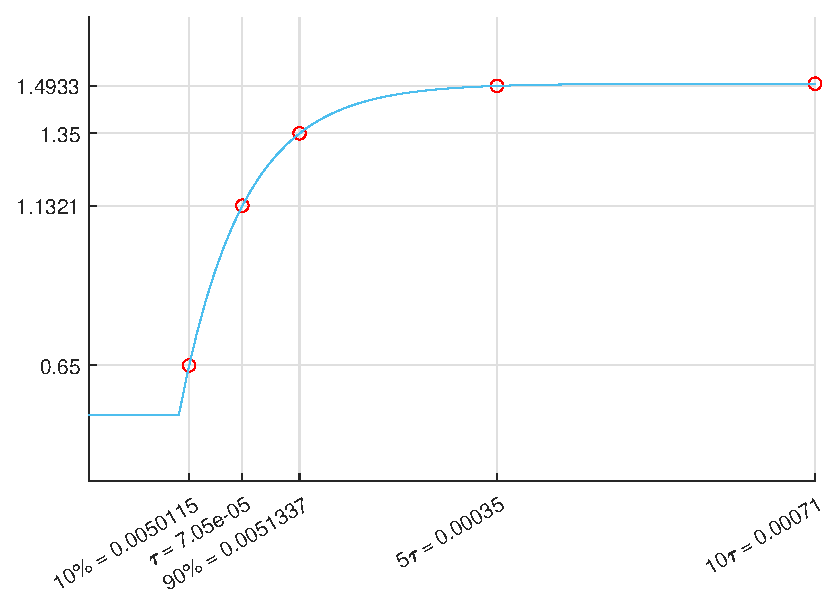
\includegraphics[width=0.9\textwidth]{../Matlab/img/CircuitA.eps}
	\caption{plot}
	\end{subfigure}	
	\hfill
	\begin{subtable}{0.38\textwidth}
		\centering
		\begin{tabular}{|c|c|c|}
			\hline
			& time [$\mu$s] & voltage [V] \\
			\hline
			$\tau$ & 70 & 1.132 \\
			\hline		
			$5\tau$ & 352 & 1.493 \\
			\hline
			$10\tau$ & 705 & 1.499 \\
			\hline
			10\% & 11 & 0.649 \\
			\hline
			90\% & 133 & 1.349 \\
			\hline
		\end{tabular}
		\caption{table of values}
	\end{subtable}
		\caption{Circuit A output voltage}
	\end{figure}
	
	\subsection{Circuit B}
	steps in circuit B are almost identical to circuit A, first we transformed circuit to s-domain according to \eqref{eq:laplace-rules}
	\begin{figure}[H]
		\centering
		\begin{circuitikz}[scale = 0.7, transform shape]
			\draw (0,0)
			to[C, l_=$\dfrac{1}{sC_{21}}$, *-] (3,0)
			to[R, l=$R_{21}$] (3,-2)
			to[short, -*] (0, -2)
			;
			\draw (0, 0) to[open, v_<=$v_{in}$] (0, -2);
			\draw (3, 0)
			to[short, -*] (5, 0)
			to[open, v^<=$v_{out}$] (5, -2)
			to[short, *-] (3, -2);
		\end{circuitikz}
		\caption{Circuit B schematics}
	\end{figure}
	
	output voltage can be described by voltage divider
	
	\begin{equation}
		V_{out}(s) = V_{in}(s) \dfrac{R_{21}}{R_{21} + \frac{1}{sC_{21}}}
	\end{equation}
	
		after applying inverse Laplace transform to $V_{out}(s)$ we obtain below plot with marked $\tau$, 5$\tau$, 10$\tau$, 10\% and 90\% of output voltage.
	
	\begin{figure}[H]
	\centering
	\begin{subfigure}{0.6\textwidth}
		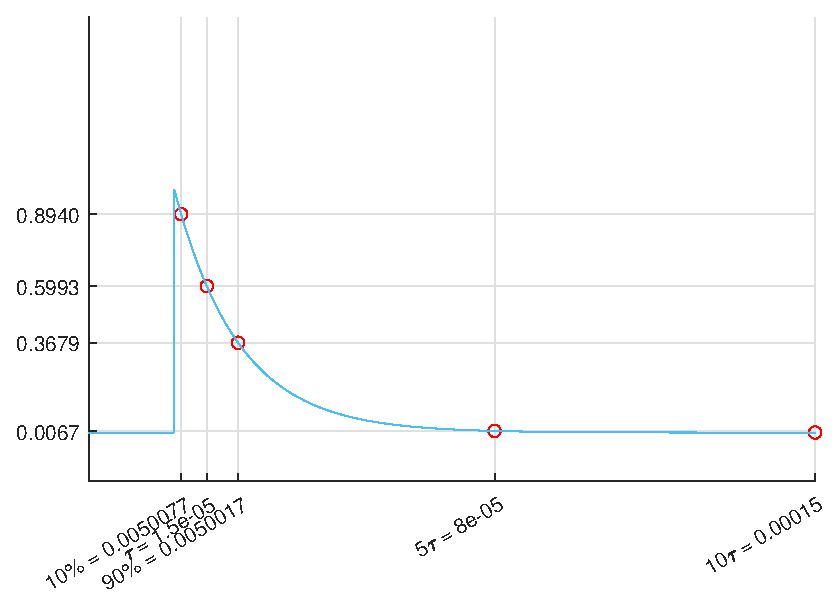
\includegraphics[width=0.9\textwidth]{../Matlab/img/CircuitB.eps}
		\caption{plot}
	\end{subfigure}
	\hfill
	\begin{subtable}{0.38\textwidth}
		\centering
		\begin{tabular}{|c|c|c|}
			\hline
			 & time [$\mu$s] & voltage [V] \\
			\hline
			$\tau$ & 15 & 0.367 \\
			\hline		
			$5\tau$ & 75 & 0.007 \\
			\hline
			$10\tau$ & 150 & 0.000 \\
			\hline
			10\% & 2 & 0.894 \\
			\hline
			90\% & 35 & 0.099 \\
			\hline
		\end{tabular}
		\caption{table of values}
	\end{subtable}
	\caption{Circuit B output voltage}
\end{figure}
	
	\subsection{Circuit C}
	
	In third circuit we are also looking for voltage of coil $L_{21}$.
	\\ \\
	Like in previous 2 circuits we transformed circuit to s-domain according to \eqref{eq:laplace-rules}
	
	\begin{figure}[H]
		\centering
		\begin{subfigure}{0.3\textwidth}
			\begin{circuitikz}[scale = 0.7, transform shape]
				\ctikzset{voltage/distance from node=.1}
				\ctikzset{voltage/bump b=2.5}
				\draw (0, 0)
				to[R, l2=$R_{in}$ and 50$\Omega$, l2 halign=c, l2 valign=b, *-] (2.5, 0)
				to[short, -*] (5, 0)
				to[open, v^<=$v_{out}$] (5, -3) -- (2.5, -3)
				to[L, l_=$sL_{41}$, v^=$V_{l3}$] (2.5, -1.5)
				to[C, l_=$\frac{1}{sC_{41}}$] (2.5, 0);
				\draw (0, 0)
				to[open, v_<=$v_{in}$](0, -3)
				to[short, -*] (2.5, -3);
			\end{circuitikz}
			\caption{JP43}
		\end{subfigure}
		\hfill
		\begin{subfigure}{0.3\textwidth}
			\begin{circuitikz}[scale = 0.7, transform shape]
				\ctikzset{voltage/distance from node=.1}
				\ctikzset{voltage/bump b=2.5}
				\draw (0, 0)
				to[R, l2=$R_{42} + R_{in}$ and 1.15k$\Omega$, l2 halign=c, l2 valign=b] (2.5, 0)
				to[short, *-*] (5, 0)
				to[open, v^<=$v_{out}$] (5, -3) -- (2.5, -3)
				to[L, l_=$sL_{41}$, v^=$V_{l2}$] (2.5, -1.5)
				to[C, l_=$\frac{1}{sC_{41}}$] (2.5, 0);
				\draw (0, 0)
				to[open, v_<=$v_{in}$](0, -3)
				to[short, -*] (2.5, -3);
			\end{circuitikz}
			\caption{JP42}
		\end{subfigure}
		\hfill
		\begin{subfigure}{0.3\textwidth}
			\begin{circuitikz}[scale = 0.7, transform shape]
				\ctikzset{voltage/distance from node=.1}
				\ctikzset{voltage/bump b=2.5}
				\draw (0, 0)
				to[R, l2=$R_{41} + R_{in}$ and 3.35k$\Omega$, l2 halign=c, l2 valign=b] (2.5, 0)
				to[short, *-*] (5, 0)
				to[open, v^<=$v_{out}$] (5, -3) -- (2.5, -3)
				to[L, l_=$sL_{41}$, v^=$V_{l1}$] (2.5, -1.5)
				to[C, l_=$\frac{1}{sC_{41}}$] (2.5, 0);
				\draw (0, 0)
				to[open, v_<=$v_{in}$](0, -3)
				to[short, -*] (2.5, -3);
			\end{circuitikz}
			\caption{JP41}
		\end{subfigure}
		\caption{Circuit C schematics}
	\end{figure}
	
	Then solved each circuit for $V_l(s)$ and $V_{out}(s)$
	
	\begin{equation}
		V_l(s) = V_{in}(s)\dfrac{sL_{41}}{R_x + \frac{1}{sC_{21}} + sL_{21}}
	\end{equation}
	
	\begin{equation}
		V_{out}(s) = V_{in}(s) \dfrac{\frac{1}{sC_{41}}+sL_{41}}{R_x + \frac{1}{sC_{41}}+sL_{41}}
	\end{equation}
	
	After plugging in value of each component where $R_x$ is series resistance of the circuit, we can transform equation back to time domain and plot results.
	
	\begin{figure}[H]
		\centering
		\begin{subfigure}{0.3 \textwidth}
			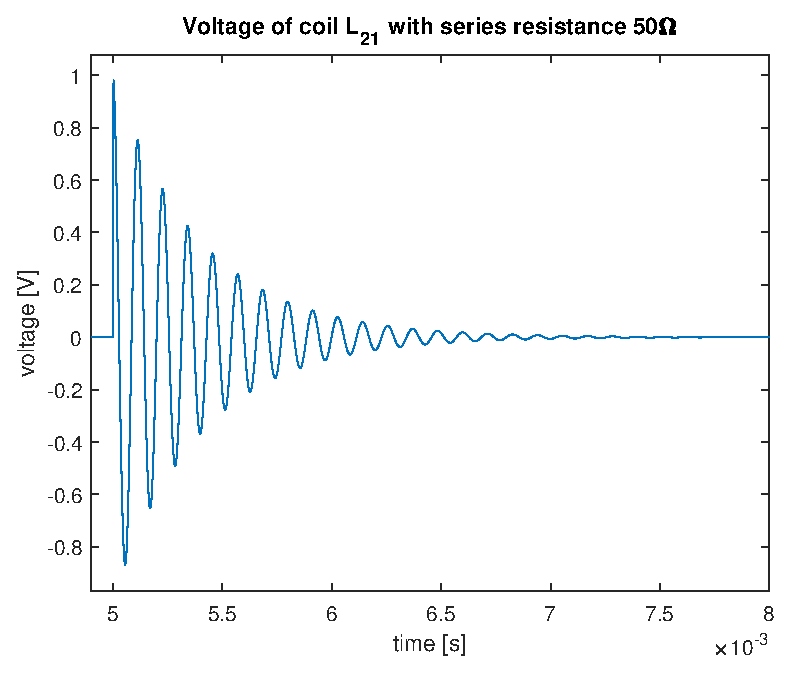
\includegraphics[width=\textwidth]{../Matlab/img/CircuitC3}
			\caption{Plot JP43}
		\end{subfigure}
		\hfill
		\begin{subfigure}{0.3 \textwidth}
			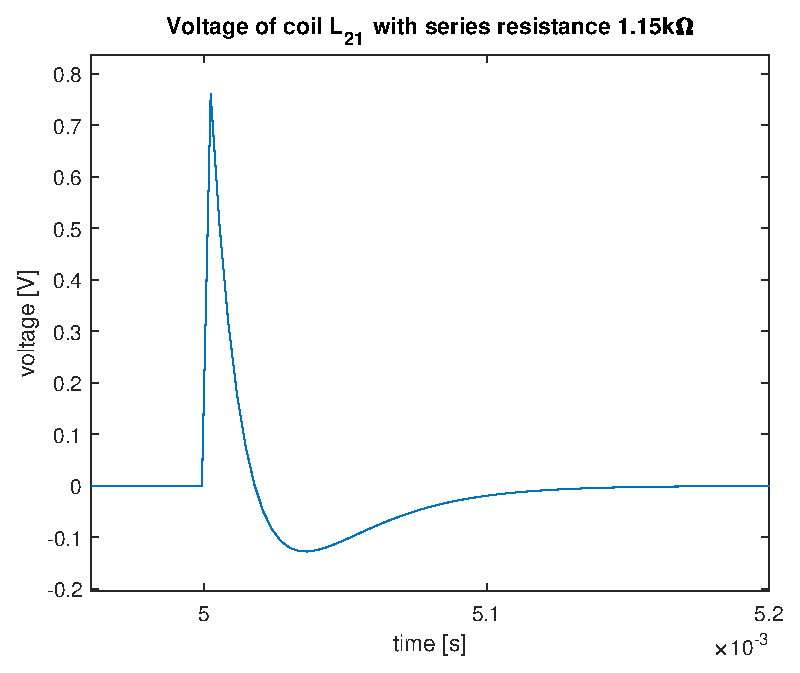
\includegraphics[width=\textwidth]{../Matlab/img/CircuitC2}
			\caption{Plot JP42}
		\end{subfigure}
		\hfill
		\begin{subfigure}{0.3 \textwidth}
			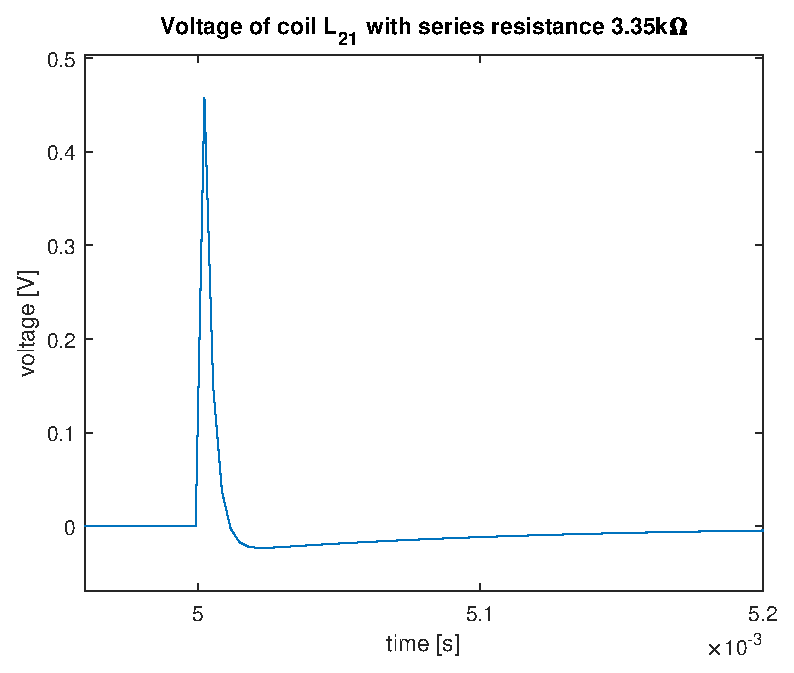
\includegraphics[width=\textwidth]{../Matlab/img/CircuitC1}
			\caption{Plot JP41}
		\end{subfigure}
				\hfill
		\begin{subtable}{0.3 \textwidth}
			\centering
			\begin{tabular}{|c|c|c|}
				\hline
				& voltage [V] & time [$\mu$s] \\
				\hline
				$v_{max}$ & 0.98 & 2 \\
				\hline
				$v_{min}$ & -0.87 & 55 \\
				\hline
				\multicolumn{2}{|c|}{ steady-state} & 1939 \\
				\hline \hline
				\multicolumn{2}{|c|}{no. of oscillations} & 18 \\
				\hline
			\end{tabular}
			\caption{Table of values JP43}
		\end{subtable}
		\hfill
		\begin{subtable}{0.3 \textwidth}
			\centering
			\begin{tabular}{|c|c|c|}
	\hline
	& voltage [V] & time [$\mu$s] \\
	\hline
	$v_{max}$ & 0.76 & 2 \\
	\hline
	$v_{min}$ & -0.127 & 36\\
	\hline
	\multicolumn{2}{|c|}{ steady-state} & 117 \\
	\hline
\end{tabular}
			\caption{Table of values JP42}
		\end{subtable}
		\hfill
		\begin{subtable}{0.3 \textwidth}
			\centering
			\begin{tabular}{|c|c|c|}
	\hline
	& voltage [V] & time [$\mu$s] \\
	\hline
	$v_{max}$ & 0.45 & 2 \\
	\hline
	$v_{min}$ & -0.023 & 24 \\
	\hline
	\multicolumn{2}{|c|}{ steady-state} & 117 \\
	\hline
\end{tabular}
			\caption{Table of values JP41}
		\end{subtable}
		\caption{Coil Voltage}
	\end{figure}
	
		\begin{figure}[H]
		\centering
		\begin{subfigure}{0.3 \textwidth}
			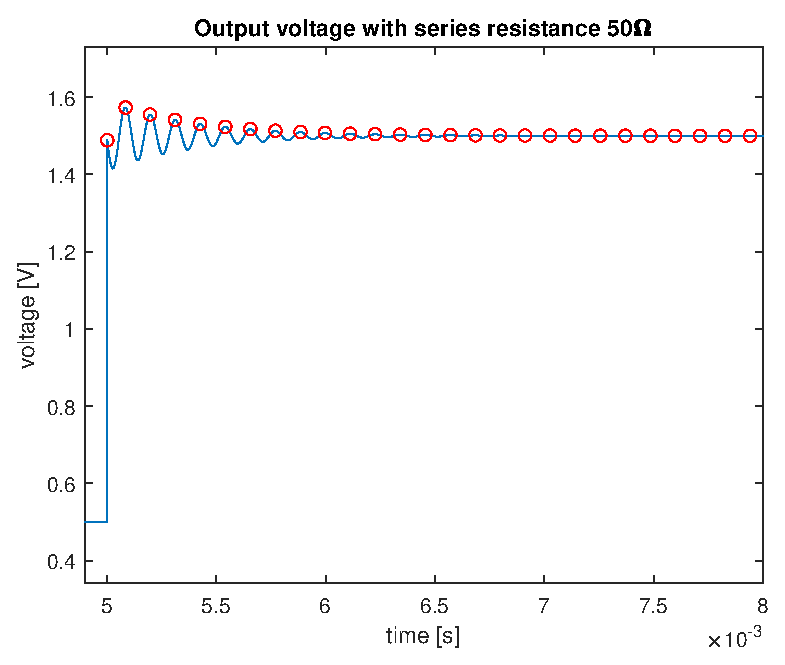
\includegraphics[width=\textwidth]{../Matlab/img/CircuitC3out}
			\caption{Plot JP43}
		\end{subfigure}
		\hfill
		\begin{subfigure}{0.3 \textwidth}
			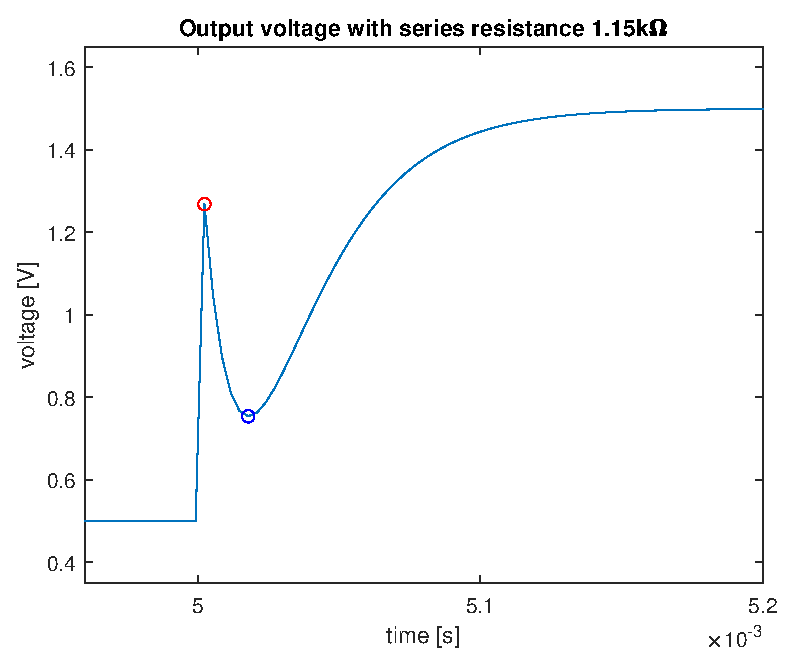
\includegraphics[width=\textwidth]{../Matlab/img/CircuitC2out}
			\caption{Plot JP42}
		\end{subfigure}
		\hfill
		\begin{subfigure}{0.3 \textwidth}
			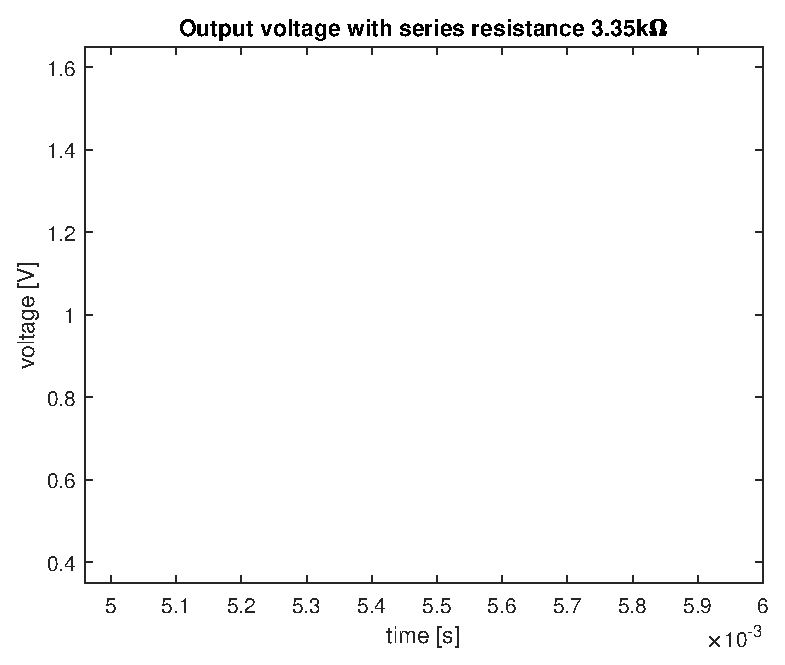
\includegraphics[width=\textwidth]{../Matlab/img/CircuitC1out}
			\caption{Plot JP41}
		\end{subfigure}
				\hfill
		\begin{subtable}{0.3 \textwidth}
			\centering
			\begin{tabular}{|c|c|c|}
	\hline
	& voltage [V] & time [$\mu$s] \\
	\hline
	$v_{max}$ & 1.57 & 86 \\
	\hline
	$v_{min}$ & 1.41 & 27\\
	\hline
	\multicolumn{2}{|c|}{ steady-state} & 885 \\
	\hline \hline
	\multicolumn{2}{|c|}{no. of oscillations} & 9 \\
	\hline
\end{tabular}
			\caption{Table of values JP43}
		\end{subtable}
		\hfill
		\begin{subtable}{0.3 \textwidth}
			\centering
			\begin{tabular}{|c|c|c|}
	\hline
	& voltage [V] & time [$\mu$s] \\
	\hline
	$v_{max}$ & 1.26 & 2 \\
	\hline
	$v_{min}$ & 0.75 & 17 \\
	\hline
	\multicolumn{2}{|c|}{ steady-state} & 144 \\
	\hline
\end{tabular}
			\caption{Table of values JP42}
		\end{subtable}
		\hfill
		\begin{subtable}{0.3 \textwidth}
			\centering
			\begin{tabular}{|c|c|c|}
	\hline
	& voltage [V] & time [$\mu$s] \\
	\hline
	$v_{max}$ & 0.96 & 2 \\
	\hline
	$v_{min}$ & 0.57 & 11 \\
	\hline
	\multicolumn{2}{|c|}{ steady-state} & 501 \\
	\hline
\end{tabular}
			\caption{Table of values JP41}
		\end{subtable}
		\caption{Output voltage}
	\end{figure}
	
	\newpage
	\section{Comparison}
	
	comparing measurements and calculations results are not very precise in every circuit, most likely by error in measurements(different offset setting) but for some circuits results differ in 3rd decimal place.
	
	\begin{figure}[H]
		\centering
		\begin{subtable}{0.45\textwidth}
			\centering
			\begin{tabular}{|c|c|c|}
			\hline
			& time [$\mu$s] & voltage [V] \\
			\hline
			$\tau$ & 70 & 1.132 \\
			\hline		
			$5\tau$ & 352 & 1.493 \\
			\hline
			$10\tau$ & 705 & 1.499 \\
			\hline
			10\% & 11 & 0.649 \\
			\hline
			90\% & 133 & 1.349 \\
			\hline
			\end{tabular}
			\caption{calculated values}
		\end{subtable}
		\hfill
		\begin{subtable}{0.45\textwidth}
			\centering
			\begin{tabular}{|c|c|c|}
				\hline
				& time [$\mu$s] & voltage [V] \\
				\hline
				$\tau$ & 64 & 0.632 \\
				\hline		
				$5\tau$ & 225 & 0.997 \\
				\hline
				$10\tau$ & 450 & 1.000 \\
				\hline
				10\% & 4 & 0.010 \\
				\hline
				90\% & 140 & 0.896 \\
				\hline
			\end{tabular}
			\caption{measured values}
		\end{subtable}
		\caption{Circuit A}
	\end{figure}	
	
	\begin{figure}[H]
		\centering
		\begin{subtable}{0.45\textwidth}
			\centering
			\begin{tabular}{|c|c|c|}
				\hline
				& time [$\mu$s] & voltage [V] \\
				\hline
				$\tau$ & 15 & 0.367 \\
				\hline		
				$5\tau$ & 75 & 0.007 \\
				\hline
				$10\tau$ & 150 & 0.000 \\
				\hline
				10\% & 2 & 0.894 \\
				\hline
				90\% & 35 & 0.099 \\
				\hline
			\end{tabular}
			\caption{calculated values}
		\end{subtable}
		\hfill
		\begin{subtable}{0.45\textwidth}
			\centering
			\begin{tabular}{|c|c|c|}
				\hline
				& time [$\mu$s] & voltage [V] \\
				\hline
				$\tau$ & 15 & 0.368 \\
				\hline		
				$5\tau$ & 73 & 0.008 \\
				\hline
				$10\tau$ & 145 & 0.000 \\
				\hline
				10\% & 1 & 0.904 \\
				\hline
				90\% & 35 & 0.100 \\
				\hline
			\end{tabular}
			\caption{measured values}
		\end{subtable}
		\caption{Circuit B}
	\end{figure}
	
	\begin{figure}[H]
		\begin{subtable}{0.45 \textwidth}
			\centering
			\begin{tabular}{|c|c|c|}
				\hline
				& voltage [V] & time [$\mu$s] \\
				\hline
				$v_{max}$ & 0.98 & 2 \\
				\hline
				$v_{min}$ & -0.87 & 55 \\
				\hline
				\multicolumn{2}{|c|}{ steady-state} & 1939 \\
				\hline \hline
				\multicolumn{2}{|c|}{no. of oscillations} & 18 \\
				\hline
			\end{tabular}
			\caption{calculated coil voltage}
		\end{subtable}
		\hfill
		\begin{subtable}{0.45 \textwidth}
			\centering
			\begin{tabular}{|c|c|c|}
				\hline
				& voltage [V] & time [$\mu$s] \\
				\hline
				$v_{max}$ & 1.02 &  \\
				\hline
				$v_{min}$ & -0.82 &  \\
				\hline
				\multicolumn{2}{|c|}{ steady-state} &  \\
				\hline \hline
				\multicolumn{2}{|c|}{no. of oscillations} &  \\
				\hline
			\end{tabular}
			\caption{measured coil voltage}
		\end{subtable}
				\begin{subtable}{0.45 \textwidth}
			\centering
			\begin{tabular}{|c|c|c|}
	\hline
& voltage [V] & time [$\mu$s] \\
\hline
$v_{max}$ & 1.57 & 86 \\
\hline
$v_{min}$ & 1.41 & 27\\
\hline
\multicolumn{2}{|c|}{ steady-state} & 885 \\
\hline \hline
\multicolumn{2}{|c|}{no. of oscillations} & 9 \\
\hline
			\end{tabular}
			\caption{calculated output voltage}
		\end{subtable}
		\hfill
		\begin{subtable}{0.45 \textwidth}
			\centering
			\begin{tabular}{|c|c|c|}
				\hline
				& voltage [V] & time [$\mu$s] \\
				\hline
				$v_{max}$ & 1.120 &  \\
				\hline
				$v_{min}$ & 0.940 &  \\
				\hline
				\multicolumn{2}{|c|}{ steady-state} & 1160 \\
				\hline \hline
				\multicolumn{2}{|c|}{no. of oscillations} & 10 \\
				\hline
			\end{tabular}
			\caption{measured output voltage}
		\end{subtable}
		\caption{Circuit C JP43}
	\end{figure}
	
		\begin{figure}[H]
		\begin{subtable}{0.45 \textwidth}
	\centering
	\begin{tabular}{|c|c|c|}
	\hline
	& voltage [V] & time [$\mu$s] \\
	\hline
	$v_{max}$ & 0.76 & 2 \\
	\hline
	$v_{min}$ & -0.127 & 36\\
	\hline
	\multicolumn{2}{|c|}{ steady-state} & 117 \\
	\hline
	\end{tabular}
	\caption{calculated coil voltage}
\end{subtable}
\hfill
\begin{subtable}{0.45 \textwidth}
	\centering
	\begin{tabular}{|c|c|c|}
		\hline
		& voltage [V] & time [$\mu$s] \\
		\hline
		$v_{max}$ & 0.920 &  \\
		\hline
		$v_{min}$ & -0.100 & \\
		\hline
		\multicolumn{2}{|c|}{ steady-state} & \\
		\hline
	\end{tabular}
	\caption{measured coil voltage}
\end{subtable}
\begin{subtable}{0.45 \textwidth}
	\centering
	\begin{tabular}{|c|c|c|}
	\hline
& voltage [V] & time [$\mu$s] \\
\hline
$v_{max}$ & 1.26 & 2 \\
\hline
$v_{min}$ & 0.75 & 17 \\
\hline
\multicolumn{2}{|c|}{ steady-state} & 144 \\
\hline
	\end{tabular}
	\caption{calculated output voltage}
\end{subtable}
\hfill
\begin{subtable}{0.45 \textwidth}
	\centering
	\begin{tabular}{|c|c|c|}
		\hline
		& voltage [V] & time [$\mu$s] \\
		\hline
		$v_{max}$ & 0.880 &  \\
		\hline
		$v_{min}$ & 0.280 & \\
		\hline
		\multicolumn{2}{|c|}{ steady-state} & \\
		\hline
	\end{tabular}
	\caption{measured output voltage}
\end{subtable}
		\caption{Circuit C JP42}
	\end{figure}
	
	\begin{figure}[H]
		\begin{subtable}{0.45 \textwidth}
	\centering
	\begin{tabular}{|c|c|c|}
	\hline
& voltage [V] & time [$\mu$s] \\
\hline
$v_{max}$ & 0.96 & 2 \\
\hline
$v_{min}$ & 0.57 & 11 \\
\hline
\multicolumn{2}{|c|}{ steady-state} & 501 \\
\hline
	\end{tabular}
	\caption{calculated coil voltage}
\end{subtable}
\hfill
\begin{subtable}{0.45 \textwidth}
	\centering
	\begin{tabular}{|c|c|c|}
		\hline
		& voltage [V] & time [$\mu$s] \\
		\hline
		$v_{max}$ & 0.721 &  \\
		\hline
		$v_{min}$ & 0.000 & \\
		\hline
		\multicolumn{2}{|c|}{ steady-state} & \\
		\hline
	\end{tabular}
	\caption{measured coil voltage}
\end{subtable}
\begin{subtable}{0.45 \textwidth}
	\centering
	\begin{tabular}{|c|c|c|}
	\hline
& voltage [V] & time [$\mu$s] \\
\hline
$v_{max}$ & 0.45 & 2 \\
\hline
$v_{min}$ & -0.023 & 24 \\
\hline
\multicolumn{2}{|c|}{ steady-state} & 117 \\
\hline
	\end{tabular}
	\caption{calculated output voltage}
\end{subtable}
\hfill
\begin{subtable}{0.45 \textwidth}
	\centering
	\begin{tabular}{|c|c|c|}
	\hline
& voltage [V] & time [$\mu$s] \\
\hline
$v_{max}$ & 0.688 & \\
\hline
$v_{min}$ & 0.064 & \\
\hline
\multicolumn{2}{|c|}{ steady-state} & \\
\hline
	\end{tabular}
	\caption{measured output voltage}
\end{subtable}
		\caption{Circuit C JP41}
	\end{figure}
	
	\section{Conclusions}
	In conclusion Laplace transform in solving circuits is excellent method which gives very accurate results, and works on algebraic level which mean that it can be calculated by a computer as we did in this exercise. Ability to simulate circuits using computer may be not necessary for small circuits but for more complex ones it is unavoidable.
	
	\newpage
	\appendix
	\section{Appendix}\label{sec:appendix}
	\href{https://github.com/kamilix2003/CT_labs}{GITHUB repository}
	\inputminted{matlab}{../Matlab/main.m}
\end{document}